\section{GPU Funktion}
I dette projekt havde jeg planer om at lave en ekstra funktion til \textit{CoreCalc} for at kunne "kode" til GPU igennem regnearket. Funktion har jeg kaldt \emph{GPU}, man skal markere de felter men vil bruge som output, ligesom funktion \textit{TRANSPOSE}. \emph{GPU} har 2 input, det første er et array, eller et data sæt, der marker det data der skal udregnes på, og det andet er et \textit{CoreCalc} udtryk/funktion, hvor talende i udtrykket peger til hvilken kolonne i den data den skal indsætte på dette placering i udregningen.

På \ref{fig:corecalc1} kan der ses et billede af \textit{CoreCalc} hvor \textit{GPU} er i brug. A1 til B6 er data sættet der vil blive brugt som input til \textit{GPU}. I C6 kan \textit{GPU} funktion beskrivelsen blive set, den tager A1 til B6 som input array (A1:B6) og et udtryk (1+2), som beskriver til \textit{GPU} at kolonne 1 skal plusse samme med kolonne 2. Bemærk at C1 til C6 er markeret mens at funktion bliver skrevet, dette bliver gjort fordi at \textit{GPU} output også er at array, så derved viser du \textit{GPU} funktion hvor dens output skal være. Bemærk at det markeret område har lige så mange rækker som input har.

\begin{figure}[p]
    \centering
    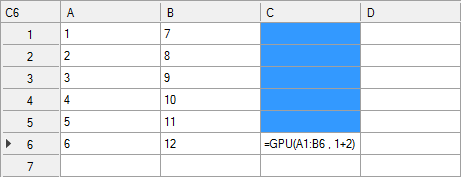
\includegraphics[width=0.8\textwidth]{Content/Graphic/corecalc1.png}
    \caption{et billede af \textit{CoreCalc} hvor \textit{GPU} bliver brugt.}
    \label{fig:corecalc1}
\end{figure}